\documentclass[10pt]{report}
\usepackage[utf8]{inputenc}
\usepackage{hyperref}
\usepackage{amssymb}
\usepackage{graphicx}
\usepackage{floatrow}
\usepackage{float}
\usepackage{listings}
\usepackage{color}
\def\euro{\mbox{\raisebox{.25ex}{{\it =}}\hspace{-.5em}{\sf C}}} 
\setcounter{secnumdepth}{5}
\setcounter{tocdepth}{5}

\newcommand{\submenu}{$\vartriangleright$}

\newcommand{\calckey}[1]{\textsf{[#1]}}
\newcommand{\calcuparrow}{\calckey{$\bigtriangleup$}}
\newcommand{\calcleftarrow}{\calckey{$\vartriangleleft$}}
\newcommand{\calcrightarrow}{\calckey{$\vartriangleright$}}
\newcommand{\calcdownarrow}{\calckey{$\bigtriangledown$}}

\lstset{
	language=bash,
	basicstyle=\scriptsize\ttfamily,
	commentstyle=\ttfamily\color{white},
	numbers=left,
	numberstyle=\ttfamily\color{white}\footnotesize,
	stepnumber=1,
	numbersep=5pt,
	backgroundcolor=\color{white},
	showspaces=false,
	showstringspaces=false,
	showtabs=false,
	frame=single,
	tabsize=2,
	captionpos=b,
	breaklines=true,
	breakatwhitespace=false,
	title=\lstname,
	escapeinside={},
	keywordstyle={\color{white}},
	morekeywords={\color{white}},
	stringstyle={\color{white}}
}



\title {TilEm2 USER MANUAL}
\author {DUPONCHELLE Thibault - MOODY Benjamin}


\begin{document}
\maketitle

\begin{figure}[H]
\centering
\scalebox{1}{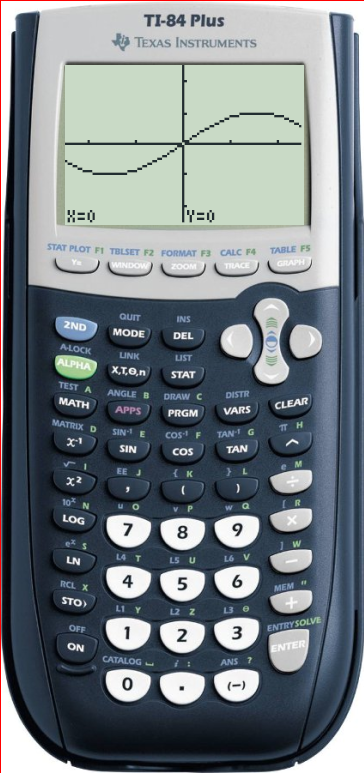
\includegraphics{pixs/tilem2.png}}
\caption{TilEm2}
\end{figure}


\tableofcontents

\chapter{Introduction}
\section{What's TilEm2?}
TilEm2 is a TI calculator emulator. It emulates all the Z80 calculators (73, 76.fr, 81, 82, 82stats, 82stats.fr, 83, 83+, 83+ SE, 84+, 84+ SE, 85, and 86) and all known ROM/OS versions.\newline
TilEm2 is completely free, and designed for Linux (but available for Windows).\newline
We put a lot of work in this software to offer to the community the best possible product.\newline
TilEm2 also provides a full featured debugger with disassembler, breakpoints, memory view and more.\newline


\section{Some history}
Some of you probably already know TilEm because a first version was released around 2000/2001 by Julien Solignac (then maintained by Benjamin Moody since 2004).\newline
This first version was working fine but there were some issues, skins were too small and bad resolution and a lot of feature were missing.\newline
Anyway, this software was pretty good (especially because the core emulation was very good).\newline

\begin{figure}[H]
\centering
\scalebox{1}{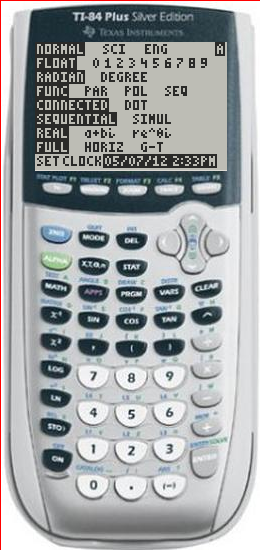
\includegraphics{pixs/tilem_old.png}}
\caption{The "old" TilEm}
\end{figure}

\begin{figure}[H]
\centering
\scalebox{1}{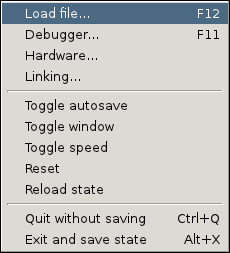
\includegraphics{pixs/tilem_old_menu.png}}
\caption{The "old" TilEm menu}
\end{figure}

We decided to rewrite this emulator from scratch, keeping the philosophy of TilEm but improving all the rest.\newline
A new core has been developped by Benjamin Moody (aka "floppusmaximus"), and I (Thibault Duponchelle aka "contra-sh") started to work on the GTK user interface (later he helped me for this task).\newline\newline
We are proud to release our work for beta testing !

\section{Features}
TilEm2 has basically all the TilEm old features plus a lot of new things :\newline
\begin{itemize}
\item   Emulates all TI z80 calc.
\item	Emulates all known rom/OS versions.
\item	Linking : Send and receive var (use libticalcs2). 
\item	Screenshot.
\item	Animated screenshot. 
\item	Grayscale. 
\item	Save states.
\item	Use TiEmu skin file format (easy to do your own skin).
\item	And more...
\end{itemize}

Here's the right click menu option :\newline
\begin{figure}[H]
\centering
\scalebox{1}{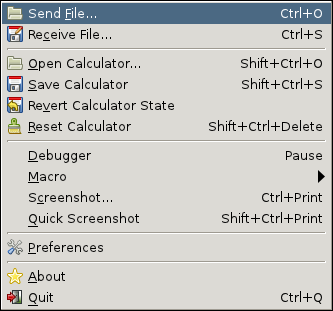
\includegraphics{pixs/popup.png}}
\caption{The right click popup menu}
\end{figure}


\section{What TilEm2 do NOT do}
TilEm2 do a lot of stuff that TilEm1 was not able to do, but there's always some feature not implemented (yet).\newline
\begin{itemize}
\item Sound handling
\item Calc to calc linking
\end{itemize}
But do not forget that developpement goes on and we are planning to do it !\newline



\section{Skins}
You can use TilEm2 without skin (just uncheck the "Use skin" checkbox into the Preferences menu) but skins are more user friendly :)\newline
We have made some officials and free to use skins (thank you to our contributors).\newline
You can do your own skins using skinedit. If you want, you can send us the skin file, maybe it could become "official".\newline\newline
What do you need to do your own skin?\newline
Just take a picture of your calc using your smartphone by example.\newline
Scale it keeping proportion to have around 900 pixels high.\newline
Then start skinedit, create a new skin, open the picture and set the key positions.\newline
It takes less than 20/30 minutes I think.\newline
See the chapter "Create your own skins" to know how to do.\newline
Then you can test it with TilEm2.That's all!\newline
Here are the current skins available by default :\newline
\begin{figure}[H]
\centering
\scalebox{1}{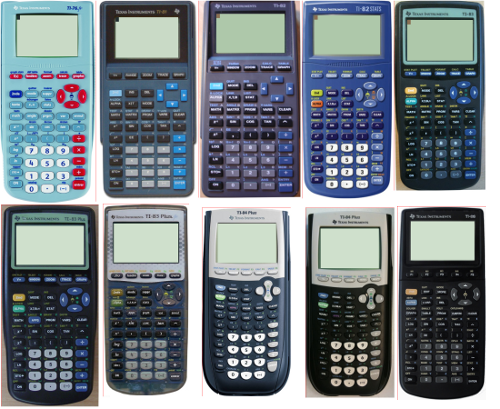
\includegraphics{pixs/diaporama_skin.png}}
\caption{The skins}
\end{figure}

\chapter{Installation}
\section{Generalities}
Before installing TilEm2, you should know that no ROM is included in this software.\newline
In order to use TilEm2, you must use your own rom (use TILP to get it).\newline
TilEm2 provides an installer msi for windows and script autoconf for Linux.\newline
There's not a lot of dependancies so you should really have no problem to install it.\newline

\section{Dependancies}
TilEm2 uses the following libraries :\newline
\begin{itemize}
\item	GTK+ 2.6 or higher (but 3.x not supported yet).
\item	libticalcs2.
\end{itemize}
You can find libticalcs2 on ticalc (from Romain Lievins).\newline

\section{Install from sources}
Download the sources of TilEm2 on sourceforge.net.\newline
Or eventually :\newline
Dowload the source from the trunk like this :\newline
\begin{lstlisting}
svn co https://tilem.svn.sourceforge.net/svnroot/tilem\newline\newline
\end{lstlisting}

Then install gtk+ (e.g. for debian : sudo apt-get install libgtk2.0-dev).\newline
Then install libticalc2.\newline\newline
(http://www.ticalc.org/archives/files/fileinfo/374/37479.html)\newline\newline

After that, simply use the configure script and the well know Linux install :\newline
\begin{lstlisting}
./configure
\end{lstlisting}
If you have no errors, so dependancies are checked and it's ok.\newline
The Makefile have been generated so type:\newline
\begin{lstlisting}
make
\end{lstlisting}
Then to copy the icons, configuration files and tilem2 binary type:\newline
\begin{lstlisting}
sudo make install
\end{lstlisting}

Usually, icons will be copied into /usr/share/tilem2/\newline
Keybindings and configuration file will be installed into \$HOME/.config/tilem2\newline

Then you can launch TilEm2 with the command :\newline
\begin{lstlisting}
tilem2 -r /path/to/rom
\end{lstlisting}

Or simply :\newline
\begin{lstlisting}
tilem2
\end{lstlisting}

\section{First use}
If you do not specify explicitely a rom on the command line, the first launch will ask you which rom you want to use.\newline
If you don't know what's a rom or how to get it, please read the chapter "Get a rom".\newline
TilEm2 will open a file chooser dialog.\newline

\begin{figure}[H]
\centering
\scalebox{1}{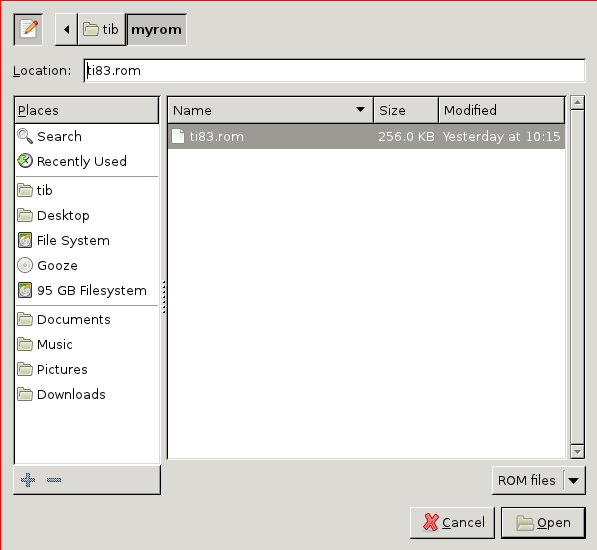
\includegraphics{pixs/first_use_rom_chooser.png}}
\caption{Starting TilEm2 for the first time}
\end{figure}

As soon you press "Ok", TilEm2 will try to guess the model of this rom (and check if it's a correct rom).\newline
When TilEm2 has a doubt, he will ask you for the model but will display only the possible candidates (not all the z80 calc).\newline
Anyway, if you launch a rom, you usually know what's model it is because as I've already said : you should have the calculator of the rom you're trying to emulate...\newline

\begin{figure}[H]
\centering
\scalebox{1}{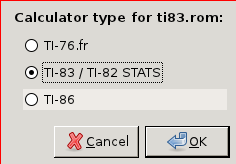
\includegraphics{pixs/first_use_model_chooser.png}}
\caption{Choose the model}
\end{figure}

After that, TilEm2 start (but calc is off you need to press on).\newline
\begin{figure}[H]
\centering
\scalebox{1}{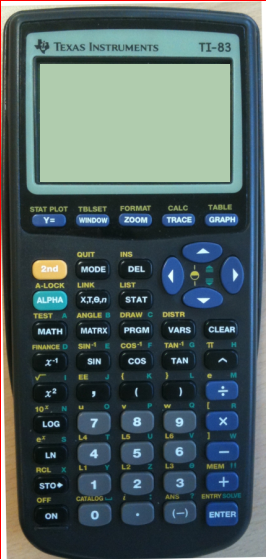
\includegraphics{pixs/first_use_works_fine.png}}
\caption{It works !}
\end{figure}
The last used rom is automatically used for the next launch of TilEm2.\newline
You can save the current state of the calculator by using "Save Calculator".\newline
If you cancel the rom chooser dialog, TilEm2 automatically shutdown.\newline

\chapter{Getting a ROM image}

In order to emulate a calculator, you must have a copy of the
calculator's operating system.  This file is referred to as a ``ROM
image,'' because, traditionally, the OS was stored in the calculator's
Read-Only Memory.  (More recent calculator models store the OS in
Flash memory instead, but the name has stuck.)

The ROM code (which forms the ``brain'' of the calculator) is
copyrighted by TI, so it is not included with TilEm.  Instead, you
will need to copy the ROM from a calculator you own.  There are
various ways to do so:

\begin{itemize}
\item For most calculator models, you can connect the calculator to
  your PC and download the ROM directly using the free software TiLP\@.

\item For the TI-83 Plus and TI-84 Plus, Andree Chea's \textsf{rom8x}
  tool allows you to copy a portion of the code from your calculator
  (using either TiLP or some other software, such as TI Graph Link or
  TI-Connect) and combine it with one of the OS upgrade files that are
  available from TI's website.

\item For the TI-81, the \textsf{dump81} package can be used to copy
  the ROM contents using a digital camera.  The other option (since
  the TI-81 has no I/O ports) is to take apart your calculator,
  desolder its ROM chip, and read the contents with an EEPROM
  programmer.
\end{itemize}

\section{Getting a ROM using TiLP}
TiLP is a free software program for communicating with TI calculators
of all types.  Like TilEm, it runs on a variety of platforms,
including Windows, Mac OS X, GNU/Linux, and FreeBSD\@.  (If you've
installed TilEm from source, you've already done most of the work of
installing TiLP\@.)  You can download TiLP from
\url{http://tilp.sourceforge.net/}.

To use TiLP, you will also need a cable to connect your calculator to
your computer.  The TI-84 Plus can be connected using a standard
mini-USB cable; for other calculators, you can either buy an official
TI Graph Link cable, or (if you're feeling adventurous) build your
own.

\subsection*{Starting TiLP}
When you launch TiLP, the main window appears:
\begin{figure}[H]
\centering
\scalebox{0.8}{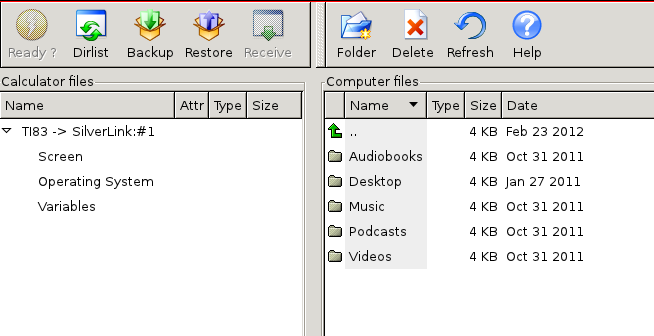
\includegraphics{pixs/tilp2_window.png}}
\caption{The TiLP main window}
\end{figure}

If it does not detect your calculator automatically, select
\textsf{File} \submenu\ \textsf{Change Device} (for older versions of
TiLP, right click on the left pane and select \textsf{Change Device}.)
Ensure that the ``Cable'' and ``Calc'' options are correct, and that
your calculator is turned on and connected.  Click the
\textsf{Dirlist} button to list the variables on your calculator, and
test whether the cable is working.

Dumping the ROM requires you to run an assembly program on your
calculator.  Although these programs have been well tested, there is
always the possibility of something going wrong, so you may want to
take this opportunity to back up any important files from your
calculator.

\subsection*{Installing a shell}
If you have a TI-73, TI-82 or TI-85, you will first need to install an
assembly shell.  These shells are not included with TilEm or TiLP, but
can be downloaded from the Web:
\begin{itemize}\raggedright
\item Mallard for the TI-73: \url{http://www.ticalc.org/pub/73/asm/shells/mallard.zip}
\item SNG for the TI-82: \url{http://www.ticalc.org/pub/82/asm/shells/sng.zip}
\item ZShell for the TI-85: \url{http://www.ticalc.org/pub/85/asm/shells/zshell.zip}
\end{itemize}

To install the shell, you will need to send a memory backup file.
Note that this replaces the entire calculator memory contents.  First,
put the calculator into link mode if necessary:
\begin{itemize}
\item On the TI-82, press
  \calckey{2nd} \calckey{X,T,$\theta$} \calcrightarrow\ \calckey{ENTER}.
\item On the TI-85, press
  \calckey{2nd} \calckey{x-VAR} \calckey{F2}.
\end{itemize}
Next, use the \textsf{Restore} option in TiLP to send the .73B, .82B,
or .85B file to your calculator.  You will need to press
\calckey{ENTER} on the TI-82, or \calckey{F1} on the TI-85, to accept
the memory backup.

\subsection*{Running the ROM dumper}
If you have a TI-82 or TI-85, put the calculator into link mode again
(using the same key sequence as above.)  Next, double-click on the
\textsf{Operating System} item in TiLP\@.  It will show a warning message:
\begin{figure}[H]
\centering
\scalebox{1}{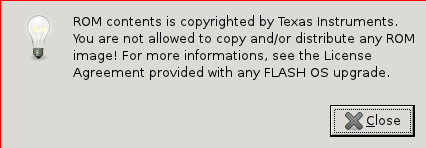
\includegraphics{pixs/tilp2_getrom_warning.png}}
\caption{The warning about the law}
\end{figure}
It will ask you again to confirm that you know what you're doing:
\begin{figure}[H]
\centering
\scalebox{1}{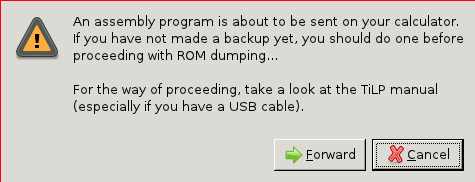
\includegraphics{pixs/tilp2_getrom_dumper.png}}
\caption{The warning before launching rom dumper}
\end{figure}

The ROM dumper will then be transferred, and if possible, launched
automatically.  On the TI-73, TI-82, or TI-85, you will need to launch
the ROM dumper manually:
\begin{itemize}
\item On the TI-73, run \textsf{prgmA} to start Mallard; ``ROM Dump''
  should already be selected, so just press \calckey{ENTER}.
\item On the TI-82, run \textsf{prgmROMDUMP}.
\item On the TI-85, press \calckey{CUSTOM} \calckey{F1} to start
  ZShell; select ``ROMDump'' and press \calckey{ENTER} to run it.
\end{itemize}

The ROM transfer will take some time\dots
\begin{figure}[H]
\centering
\scalebox{1}{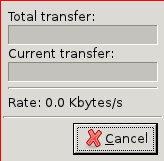
\includegraphics{pixs/tilp2_getrom_transfert.png}}
\caption{The transfert}
\end{figure}

\chapter{Main features}

In addition to emulate the behaviour of a real calc, TilEm2 features main functionnalities as file loading and file export, screenshot, debugger.\newline
In this chapter, we will talk about these main features.\newline
In an another chapter, yoou will find a detailled explanation of all options of TilEm2.\newline

\section{Send a file from PC to TilEm2}

Here we talk about sending a file from computer to emulated calc.\newline
You downloaded a file on the web and you want to test it before sending it to your calc?\newline
You compiled a file and you want to see the result?\newline
So you probably want to use send file feature...\newline\newline
There's 3 ways to do that.\newline

\subsection{Using the right click menu option}

Firstly right click on the calc.\newline
This menu popup will appear : \newline
\begin{figure}[H]
\centering
\scalebox{1}{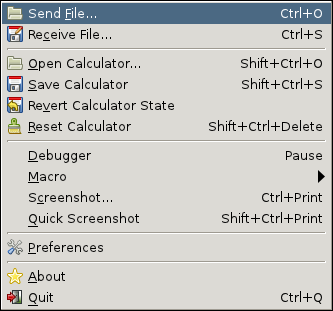
\includegraphics{pixs/send_file.png}}
\caption{The "Send File..." menu entry}
\end{figure}
Click on Send file...\newline
(You can bypass the popup menu by clicking CTRL + O)\newline
\begin{figure}[H]
\centering
\scalebox{1}{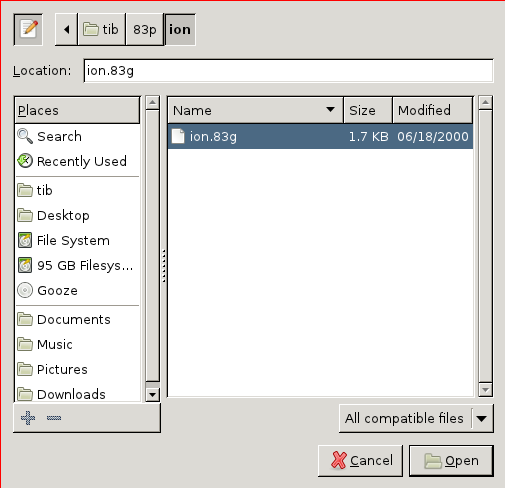
\includegraphics{pixs/send_file_chooser.png}}
\caption{The "Send File..." file chooser dialog}
\end{figure}
Then explore your computer and choose the file(s) you want to send.\newline
Usually, variable are suffixed by something like .82p (ti82), .83p (ti83) .8xp (ti83+, ti84+), .86p (ti86) or something else.\newline
Grouped files are generally suffixed by .82g (ti82), .83g (ti83), .8xg (ti83+, ti84+).86g (ti86) or something else.\newline
Some other special extension as .8kv are flashapp for ti83+, ti84+.\newline
And a lot of other file extension.\newline

It could take some time to load a variable so a current progress bar is printed while loading to know what's happening.\newline

As soon as you press OK, the file start to be loaded and a progress bar is displayed.\newline

\begin{figure}[H]
\centering
\scalebox{0.5}{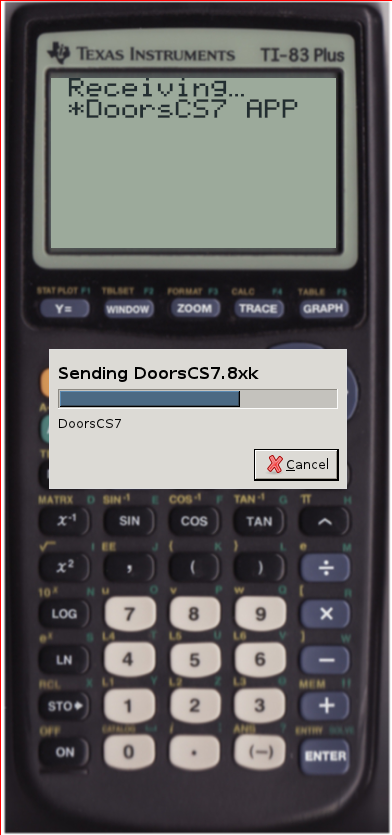
\includegraphics{pixs/send_file_loading.png}}
\caption{The "Senf File..." progress bar update}
\end{figure}


\subsection{Using drag and drop}
Simply select one or more files on your computer and use drag and drop to

\begin{figure}[H]
\centering
\scalebox{0.3}{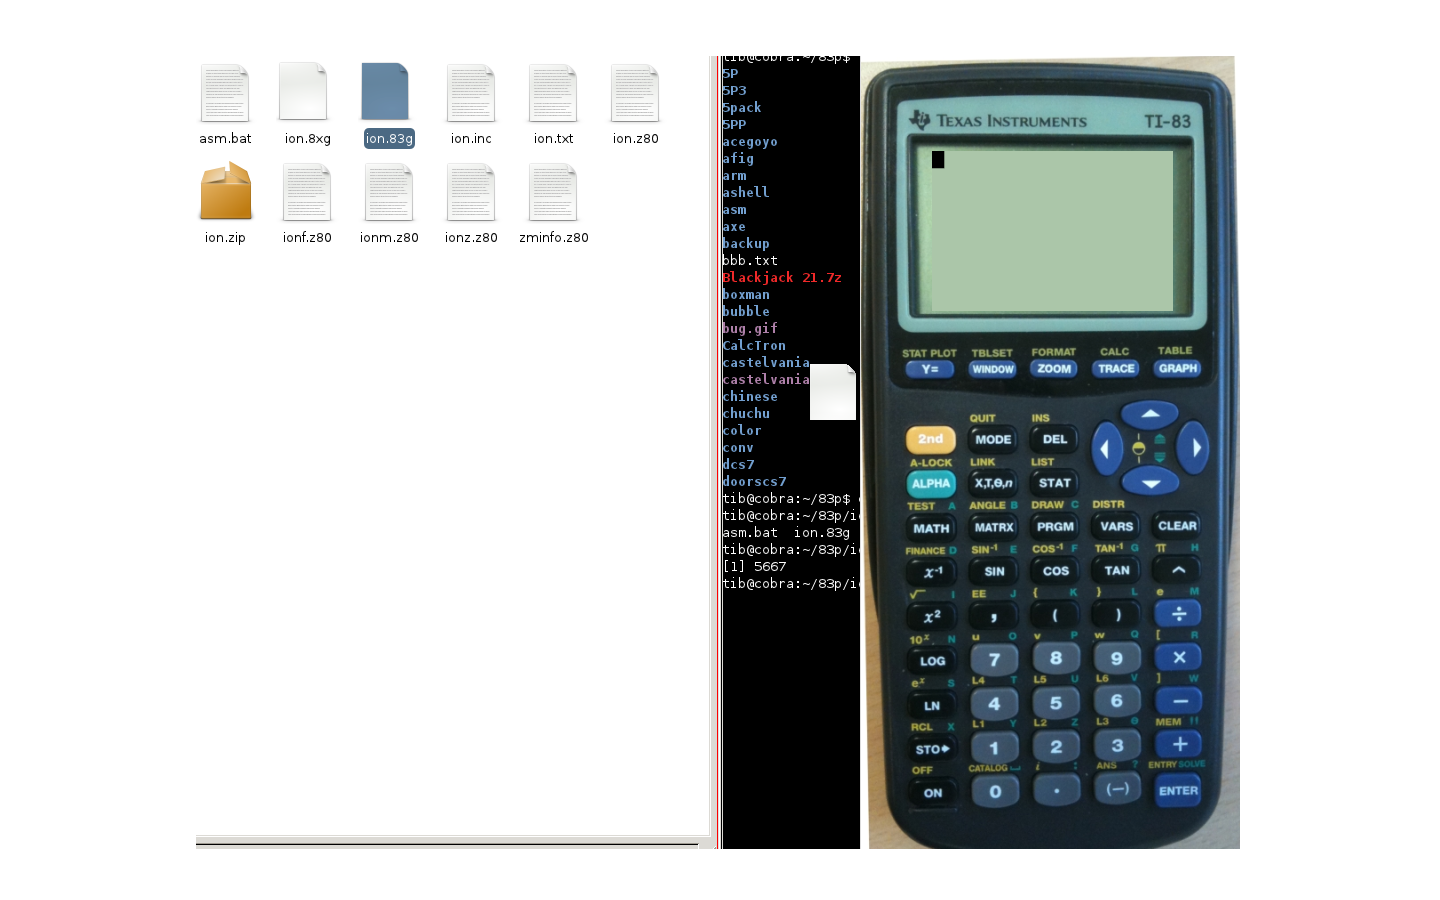
\includegraphics{pixs/send_file_drag_and_drop.png}}
\caption{Drag and Drop}
\end{figure}

You will not see any visual feedback (no progress bar) but you can see in your terminal eventually the libticalcs debugging messages.\newline

\begin{figure}[H]
\centering
\scalebox{0.3}{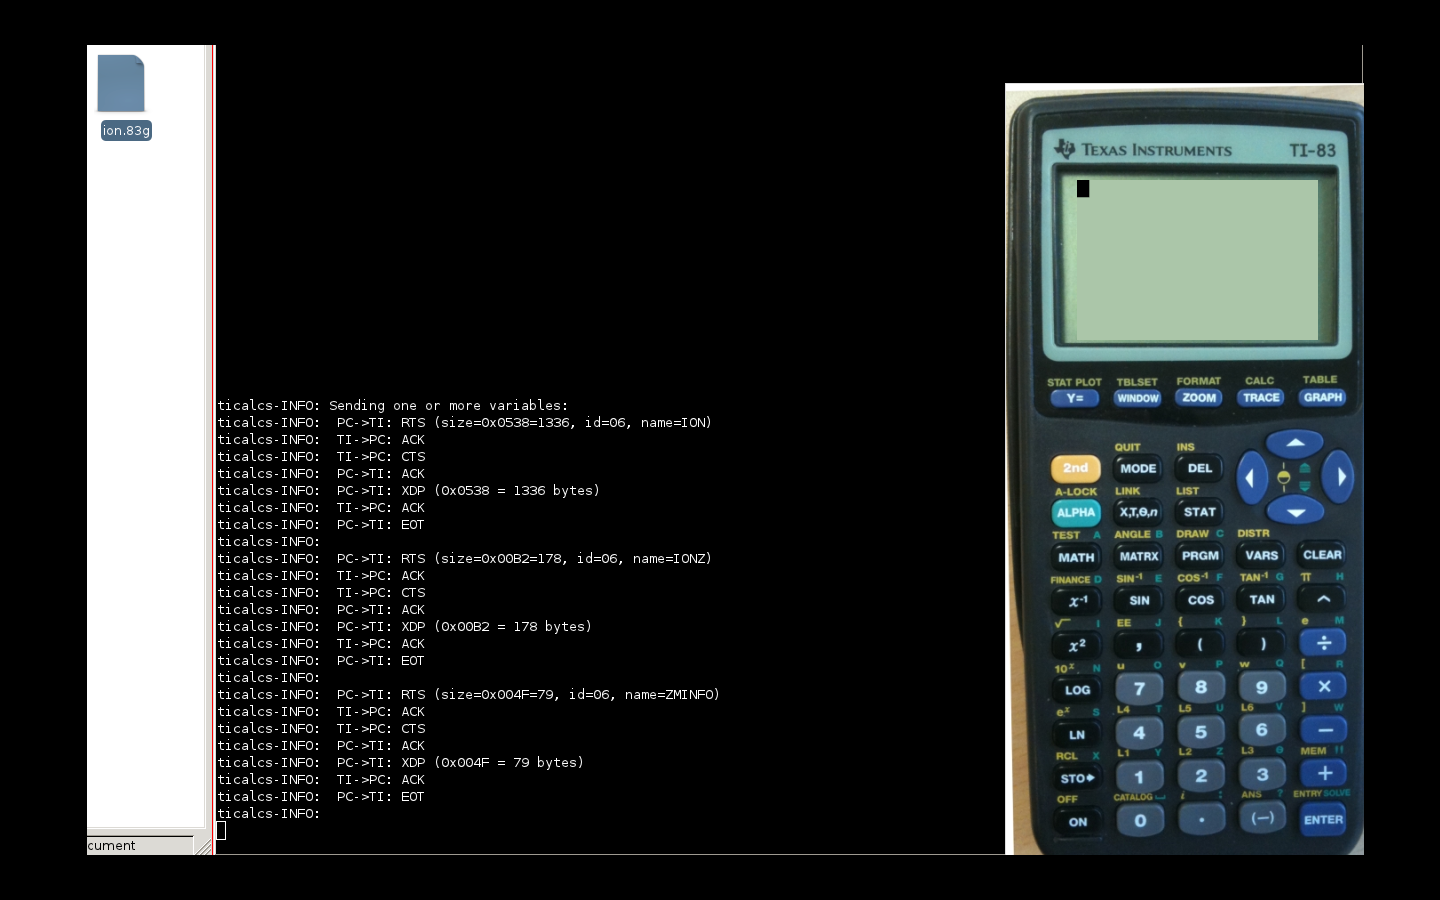
\includegraphics{pixs/send_file_drag_and_drop_libticalcs.png}}
\caption{Drag and Drop}
\end{figure}


You can check if your program is correctly uploaded to calc by listing them inside the program menu (if it's a program) :
\begin{figure}[H]
\centering
\scalebox{0.5}{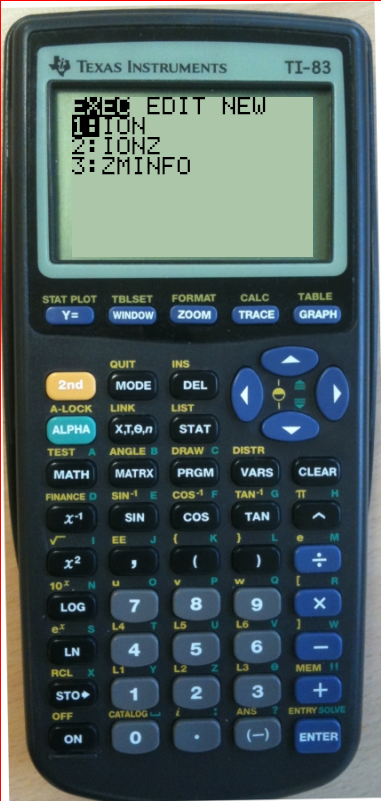
\includegraphics{pixs/send_file_list.png}}
\caption{Check if a programs is uploaded correctly (here on a ti83)}
\end{figure}

\subsection{Using the command line}

You can also send a file to the calc at startup using command line parameters.\newline
All the non options args are sent to the calc.\newline

\begin{lstlisting}
tilem2 -r $rom ion.83g
\end{lstlisting}
This example will load the group file ion.83g in the calc memory.\newline

\section{Get a var from calc to PC}

To get a program, list, screen, application or whatever which is considered are a var on the calc you need to use the right click menu options :\newline
(Or you can simply use CTRL + S)\newline

\begin{figure}[H]
\centering
\scalebox{0.5}{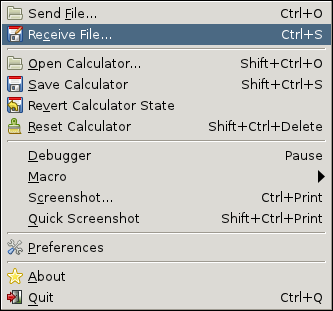
\includegraphics{pixs/receive_file.png}}
\caption{The "Receive File..." dialog}
\end{figure}

At this point, TilEm2 will (try to) get the variables and print them into a list.\newline
This is why you will see the progress bar.\newline
Warning : update is not done each time the window is popup, you need to refresh manually the vars.\newline\newline
You can select one or more vars in the list then saving it by clicking "Save".\newline
\begin{figure}[H]
\centering
\scalebox{0.5}{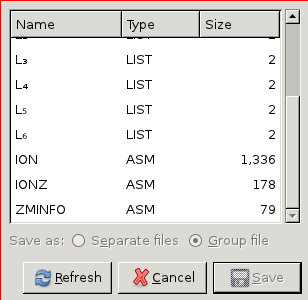
\includegraphics{pixs/receive_file_list.png}}
\caption{Listing the variables}
\end{figure}

A check button lets you choose the format of the output.\newline
If you want to get more than one var, you can save it as grouped file or as separate files (separate files is as you get it one by one).\newline

\begin{figure}[H]
\centering
\scalebox{0.5}{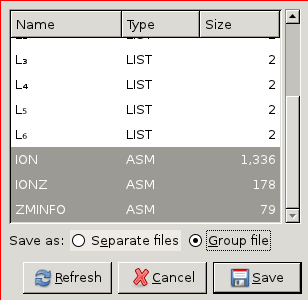
\includegraphics{pixs/receive_file_separate_or_grouped.png}}
\caption{Listing the variables}
\end{figure}

Then simply click save and choose a place to backup the var(s).\newline


\section{Record or grab a screenshot}

As screenies are a good way to show your projects or whatever you want, TilEm2 provide a complete screenshot dialog.\newline
We think this dialog to be user friendly and powerful.\newline
There's also a special manner to quickly screenshoot the lcd content ("Quick Screenshot" or SHIFT + CTRL + PRINT).\newline
We will describe this method in a first subsection then we will talk about more powerful methods.\newline

\subsection{Grab a screenshot using "Quick Screenshot"}

You can grab a screenshot without using screenshot dialog.\newline
Simply click on the "Quick Screenshot" menu option or SHIFT + CTRL + PRINT.\newline
The screenshot use the default options (or the options you have given into screenshot dialog).\newline
The picture is stored into the directory you usually use for screenshot OR if not exists into the ~/.config/tilem2/screenshots/ or equivalent if you're not on Linux.\newline

\begin{figure}[H]
\centering
\scalebox{0.5}{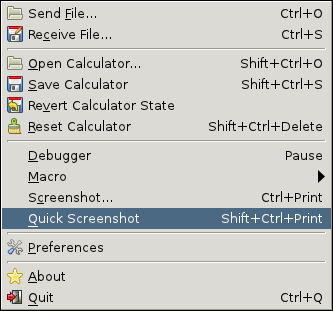
\includegraphics{pixs/quick_screenshot.png}}
\caption{The "Quick Screenshot" submenu}
\end{figure}

\subsection{Grab a screenshot using the screnshot dialog}

Click on "Screenshot" menu option or use CTRL + PRINT.\newline
\begin{figure}[H]
\centering
\scalebox{0.5}{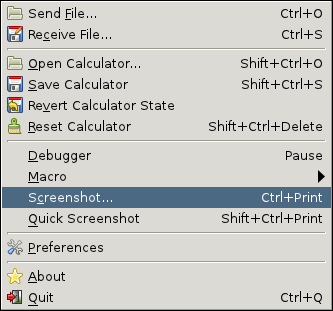
\includegraphics{pixs/screenshot.png}}
\caption{The "Screenshot..." submenu}
\end{figure}

The screenshot window will open.\newline
TilEm2 automatically grab a screenshot at startup.\newline
\begin{figure}[H]
\centering
\scalebox{0.5}{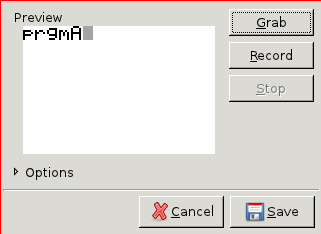
\includegraphics{pixs/screenshot_dialog_grab.png}}
\caption{The window opens with a first grabed screenshot}
\end{figure}

You can choose to "Save" it or to grab another screenshot.\newline
There's a lot of options as size, foreground/background color etc...\newline
\begin{figure}[H]
\centering
\scalebox{0.5}{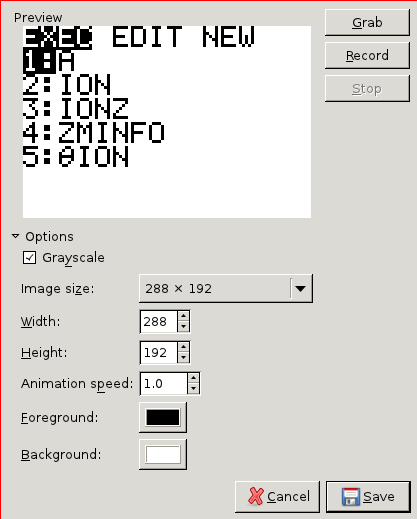
\includegraphics{pixs/screenshot_dialog.png}}
\caption{The options}
\end{figure}

There's some differents kind of output format as png, bmp or some other else.\newline

\subsection{Record a gif}

Click on "Screenshot" menu option or use CTRL + PRINT.\newline
\begin{figure}[H]
\centering
\scalebox{0.5}{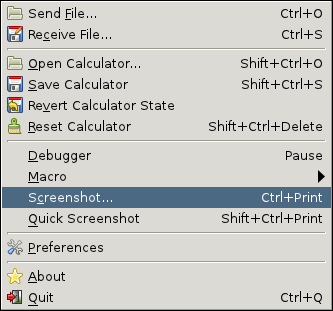
\includegraphics{pixs/screenshot.png}}
\caption{The "Screenshot..." submenu}
\end{figure}

The screenshot window will open.\newline
\begin{figure}[H]
\centering
\scalebox{0.5}{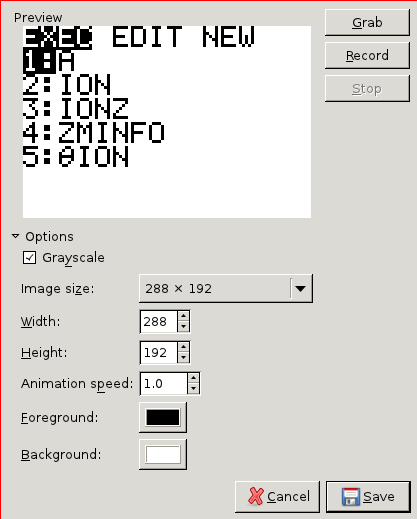
\includegraphics{pixs/screenshot_dialog.png}}
\caption{The "Screenshot" window}
\end{figure}

You can record a gif by clicking "Record".\newline
Stop the gif by clicking "Stop" (What a surprise :D).\newline
As soon you click "Stop", a preview is available in the picture area.\newline
There's a lot of options as size, foreground/background color etc...\newline
You can set these options after recording the animation.\newline

When you have the desired animation, clickon "Save" button and choose a place and a filename to save the gif.\newline

\subsection{Screenshot options}

Static screenshots and animated screenshots both use settings. Here's how to use these seetings.\newline

\paragraph{Size}


You can choose between "default" size for the screenies :\newline
7 default size for the TI-86 and 3 for the other models.\newline

\begin{figure}[H]
\centering
\scalebox{0.5}{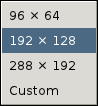
\includegraphics{pixs/screenshot_widget_size_list.png}}
\caption{The "Size" listbox for all models except TI-86}
\end{figure}

For the TI-86, ratio and values proposed by default are different: \newline

\begin{figure}[H]
\centering
\scalebox{0.5}{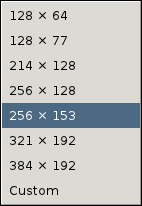
\includegraphics{pixs/screenshot_widget_size_list_86.png}}
\caption{The "Size" listbox for TI-86}
\end{figure}

Default values are proposed to help you to choose correct ratio (the choice depends on the size of the lcd).\newline

Here's what you have for all models except TI-86 :\newline
\begin{itemize}
\item 96 x 64
\begin{figure}[H]
\centering
\scalebox{0.5}{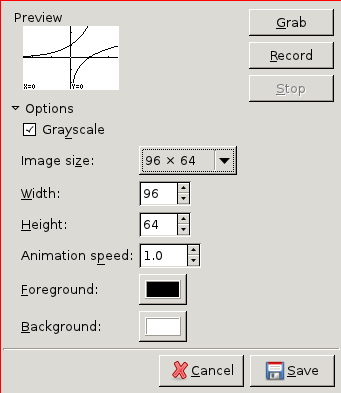
\includegraphics{pixs/screenshot_grab_small.png}}
\caption{Small (or normal)}
\end{figure}
\item 192 x 128
\begin{figure}[H]
\centering
\scalebox{0.5}{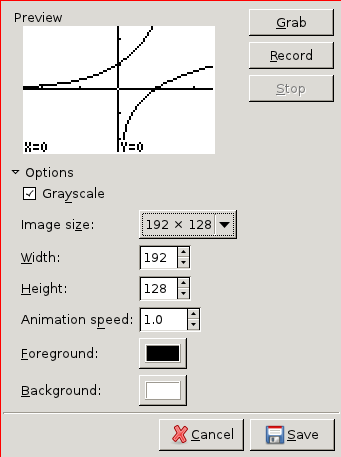
\includegraphics{pixs/screenshot_grab_medium.png}}
\caption{Medium}
\end{figure}
\item 288 x 192
\begin{figure}[H]
\centering
\scalebox{0.5}{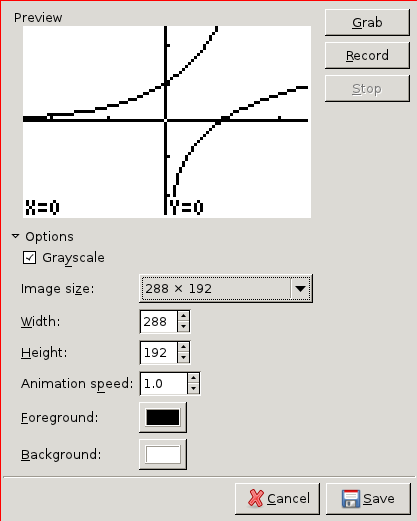
\includegraphics{pixs/screenshot_grab_big.png}}
\caption{Big}
\end{figure}
\end{itemize}

I will not show the same screenshot for the TI-86 it's not necessary.\newline

This is "default" sized screenies but you can set your own (warning : try to keep the ratio).\newline
Setting your own size could produce some curious results (here the biggest possible) :\newline
\begin{figure}[H]
\centering
\scalebox{0.5}{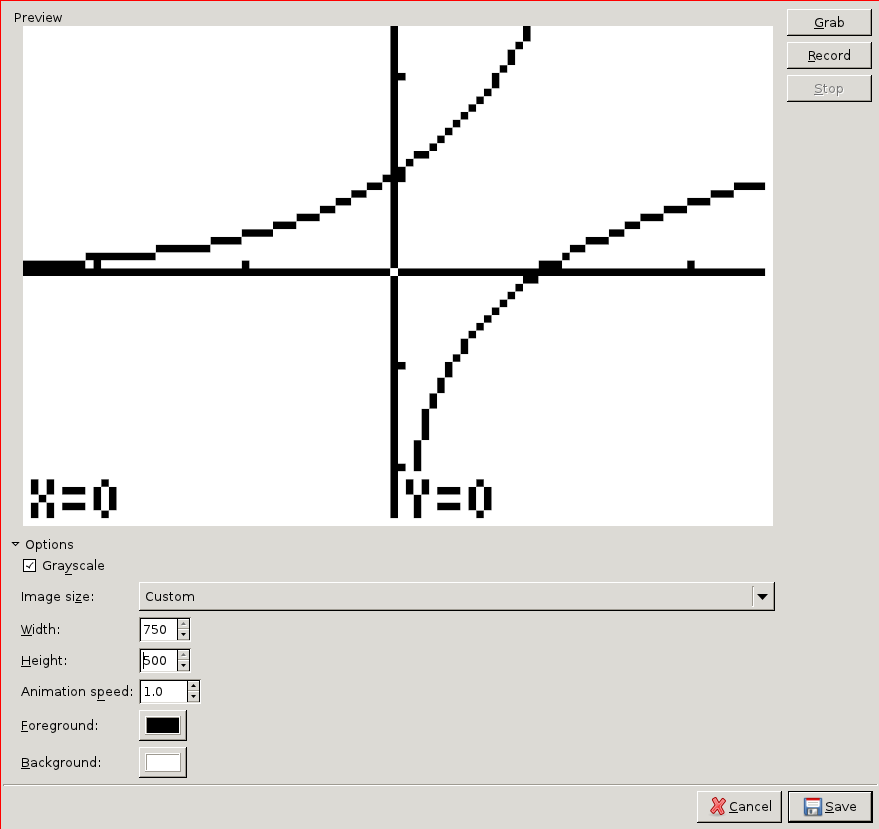
\includegraphics{pixs/screenshot_grab_huge.png}}
\caption{Huge !}
\end{figure}

\paragraph{Animation speed}

There's a setting called "Animation speed" which is used by the animated screenies.\newline
If you increment this value, the animation will run faster.\newline
A visual feedback will show you the effect of increasing this value.\newline
The max is set to 100.\newline
\begin{figure}[H]
\centering
\scalebox{0.5}{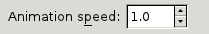
\includegraphics{pixs/screenshot_widget_animation_speed.png}}
\caption{The "Animation speed" widget}
\end{figure}


\paragraph{Foreground and background colors}

Below the "animation speed" there's 2 color chooser which allow you to set your own colors for foreground and background colors (as you know z80 calc LCD is monochrome).\newline

\begin{figure}[H]
\centering
\scalebox{0.5}{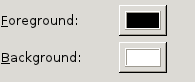
\includegraphics{pixs/screenshot_widget_color_chooser.png}}
\caption{The "Color chooser" widget}
\end{figure}

The grayscales screenies are fully compatible with this setting of course (because it's no more than "flashing").\newline
Here's a sample of what you get if you choose a pink as foreground color and green as background color :\newline
\begin{figure}[H]
\centering
\scalebox{0.5}{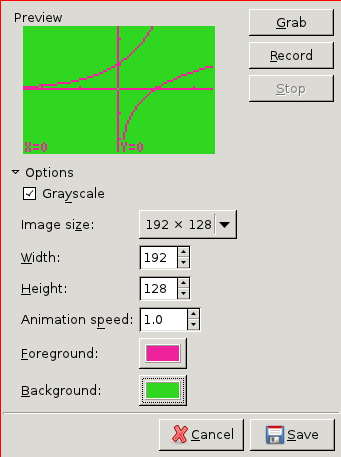
\includegraphics{pixs/screenshot_grab_color.png}}
\caption{Colored screenshot}
\end{figure}

Let's see a bunch of colored screenies:\newline
\begin{figure}[H]
\centering
\scalebox{0.5}{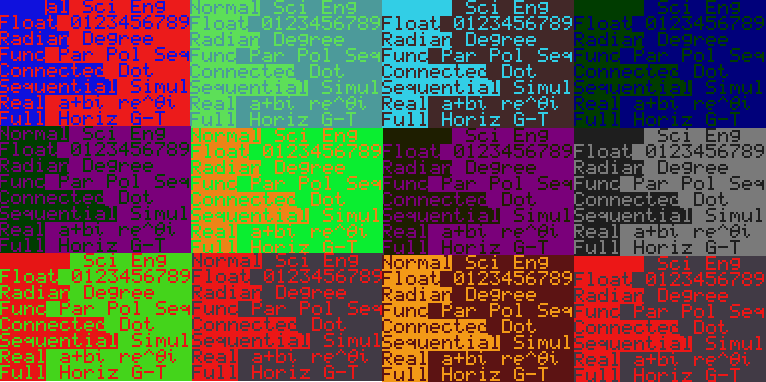
\includegraphics{pixs/screenshot_color_diaporama.png}}
\caption{Some other samples}
\end{figure}

Of course these settings are usually used to correct contrast or simply set a better color ratio (not to do the useless but funny screenshots I've shown just before).\newline

\paragraph{Grayscale}


\begin{figure}[H]
\centering
\scalebox{0.5}{
\includegraphics{pixs/screenshot_widget_grayscale.png}}
\caption{The "Grayscale" checkbox}
\end{figure}

A last setting called "Grayscale" let you choose the rendering mode.\newline
%%%% Benjamin could you talk about grayscale checkbox here %%%

\section{Use the debugger}
This is an important part of an emulator...\newline
The debugger provide an easy way to inspect the core of the calc and to find bugs into your projects.\newline

\subsection{General presentation}

When you start the debugger (using "Pause" or the right click menu entry) 
\begin{figure}[H]
\centering
\scalebox{0.5}{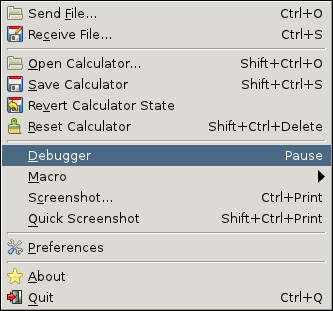
\includegraphics{pixs/debugger.png}}
\caption{The "Debugger" menu entry}
\end{figure}

The calc will be paused automatically (you can't work with debugger while calc is running that's evident).\newline
If you click on F5 to run the calc the emulator will be deactivated to prevent to edit anything in the debugger.\newline
You can pause the calc by clicking ESC (escape).\newline
\begin{figure}[H]
\centering
\scalebox{0.5}{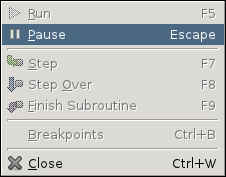
\includegraphics{pixs/debugger_pause.png}}
\caption{The "Pause" menu entry (Debug menu)}
\end{figure}

Or by using the "Pause" button (tool bar behind the menu bar).\newline
\begin{figure}[H]
\centering
\scalebox{0.5}{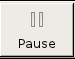
\includegraphics{pixs/debugger_pause_button.png}}
\caption{The "Pause" button}
\end{figure}

The aim of the debugger is to show the disasm memory, the registers, stack and the memory.\newline
The values are written in hexadecimal format.Not decimal.\newline
What does it mean?\newline
Simply one little sample :\newline
increment 0 = 1;\newline
increment 1 = 2;\newline
increment 2 = 3;\newline
increment 3 = 4;\newline
increment 4 = 5;\newline
increment 5 = 6;\newline
increment 6 = 7;\newline
increment 7 = 8;\newline
increment 8 = 9;\newline
increment 9 = A;\newline
increment A = B;\newline
increment B = C;\newline
increment C = D;\newline
increment D = E;\newline
increment E = F;\newline
increment F = 10;\newline
Ok we will not explain more the hexadecimal format, just accept the fact that's in hexadecimal format.\newline
For a large part of TilEm2 users, hexadecimal is not a surprise :)\newline\newline
Let's talk about widget organization.\newline


\subsection{Widget organization}

There's at least 6 zones into this window :\newline
\begin{itemize}
\item The menu bar :\newline
\begin{figure}[H]
\centering
\scalebox{0.8}{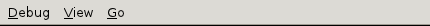
\includegraphics{pixs/debugger_menu_bar.png}}
\caption{The menu bar}
\end{figure}
\item The button bar :\newline
\begin{figure}[H]
\centering
\scalebox{0.8}{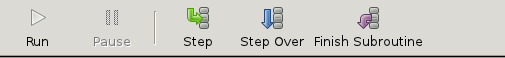
\includegraphics{pixs/debugger_button_bar.png}}
\caption{The button bar}
\end{figure}
\item The disasm view :\newline
\begin{figure}[H]
\centering
\scalebox{0.8}{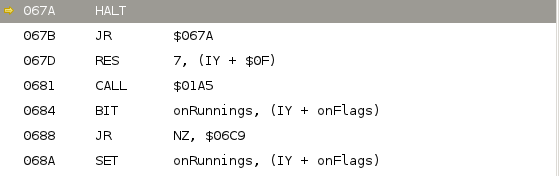
\includegraphics{pixs/debugger_disasm_view.png}}
\caption{The disasm view}
\end{figure}
\item The memory view :\newline
\begin{figure}[H]
\centering
\scalebox{0.8}{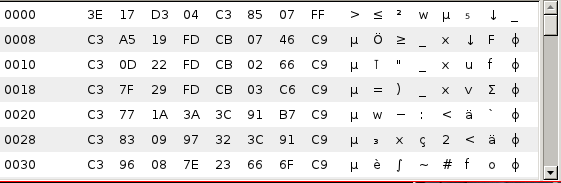
\includegraphics{pixs/debugger_memory_view.png}}
\caption{The memory view}
\end{figure}
\item The register view :\newline
\begin{figure}[H]
\centering
\scalebox{0.8}{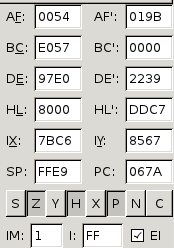
\includegraphics{pixs/debugger_register_view.png}}
\caption{The register view}
\end{figure}
\item The stack view :\newline
\begin{figure}[H]
\centering
\scalebox{0.8}{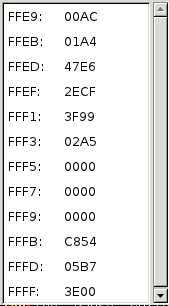
\includegraphics{pixs/debugger_stack_view.png}}
\caption{The stack view}
\end{figure}
\end{itemize}

All this view produce the debugger (there's some other window hidden by example breakpoints dialog and keypad window).\newline
\begin{figure}[H]
\centering
\scalebox{0.5}{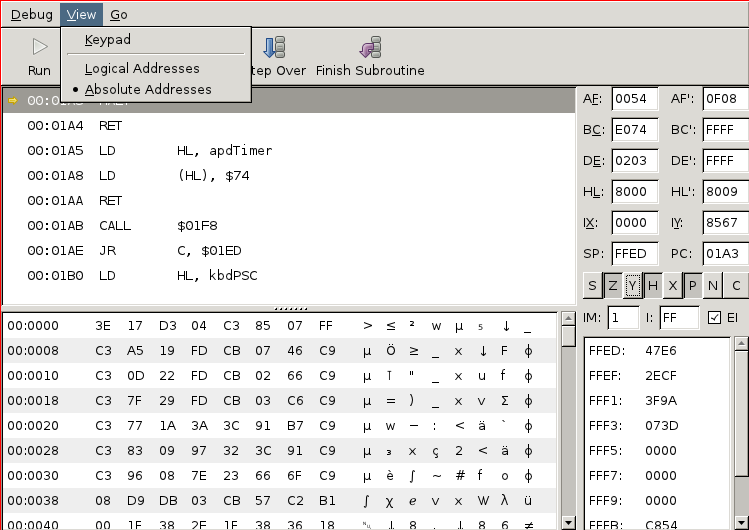
\includegraphics{pixs/debugger_view.png}}
\caption{The debugger}
\end{figure}

\subsection{Use the disasm view}

As you probably know, there's a register which store the adress of the current instruction.\newline
It's called PC ("Program Counter").\newline
If you look into the value of PC, you should recognize that the value is the same as the adress pointed by a yellow arrow in the disasm.\newline 
This is the current instruction which is executed.\newline
See this example :\newline
\begin{figure}[H]
\centering
\scalebox{0.5}{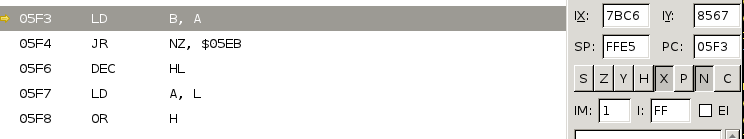
\includegraphics{pixs/debugger_pc_equal_current_instruction.png}}
\caption{The value of PC is 05F3 as the adress of the current instruction}
\end{figure}

As you may know, even if z80 is most like "RISC" methodology (in the sense the mnemo are pretty simple and fast) the size of the instruction depends the instruction itself.\newline
That's why the adress are not linearly incremented.\newline
Sometimes an instruction is stored on 1 byte, sometimes 2 bytes, sometimes 3 bytes etc...\newline

A sample for 1 byte sized instruction :\newline
\begin{figure}[H]
\centering
\scalebox{0.8}{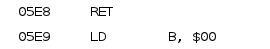
\includegraphics{pixs/debugger_instruction_1bytes.png}}
\caption{Only one byte for RET}
\end{figure}

A sample for 2 bytes sized instruction :\newline
\begin{figure}[H]
\centering
\scalebox{0.8}{\includegraphics{pixs/debugger_instruction_2bytes.png}}
\caption{2 bytes...}
\end{figure}

A sample for 3 bytes sized instruction :\newline
\begin{figure}[H]
\centering
\scalebox{0.8}{\includegraphics{pixs/debugger_instruction_3bytes.png}}
\caption{3 bytes...}
\end{figure}

This view show the disasm memory, so you can see the entire memory, but not as hexadecimal value but as assembly mnemos.\newline
As you can see, some values are replaced by their symbols.
\begin{figure}[H]
\centering
\scalebox{0.8}{\includegraphics{pixs/debugger_replaced_symbol.png}}
\caption{The value is replaced by its symbol}
\end{figure}

This is not a default behavious of a z80 debugger, so that's the job of an equate file loaded by TilEm2 at startup (files called .sym into the data directory).\newline
In fact that's just adress values replaced by a label (for human readable purpose).\newline
Exactly as you use an equate file instead of calling directly the adress for a call.\newline
When you use "call BUFCOPY" (ti83), you don't want to see the exact value of this jump.\newline

Always about the disasm view, you can "Goto adress..." : \newline
Using right click on the disasm view : \newline
\begin{figure}[H]
\centering
\scalebox{0.8}{\includegraphics{pixs/debugger_goto_adress.png}}
\caption{The "Goto adress..." right click menu entry.}
\end{figure}

Or using the "Go" menu into the menu bar :\newline
\begin{figure}[H]
\centering
\scalebox{0.8}{\includegraphics{pixs/debugger_go.png}}
\caption{The "Go" menu.}
\end{figure}

\begin{figure}[H]
\centering
\scalebox{0.8}{\includegraphics{pixs/debugger_goto_adress_menu.png}}
\caption{The "Goto adress..." from the go menu}
\end{figure}

This option lets you choose an adress to "jump" (only user interface no action on the calc).\newline
Because it can be very annoying to scroll the disasm view.\newline

\begin{figure}[H]
\centering
\scalebox{0.8}{\includegraphics{pixs/debugger_goto_adress_input.png}}
\caption{Enter the adress...}
\end{figure}
One more time : "Goto adress" doesn't change anything to the "PC" or whatever.\newline 

You can also use CTRL + L to do this task without using the mouse.\newline

Another option is to jump to the "PC". It's like goto adress, but without prompting an adress, it will jump to the "PC" directly.\newline

Using it from the menu bar ("Go" menu) : \newline
\begin{figure}[H]
\centering
\scalebox{0.8}{\includegraphics{pixs/debugger_current_pc_menu.png}}
\caption{The "Goto adress..." from the go menu}
\end{figure}

Or right click on the disasm view :\newline
\begin{figure}[H]
\centering
\scalebox{1}{\includegraphics{pixs/debugger_current_pc.png}}
\caption{The "Goto adress..." from the go menu}
\end{figure}

Now let's talk about interactivity.\newline
As you can see, a a lot of informations are updated each time the calc run (or do a step).\newline
Stack, registers, and memory is updated in the same time the disasm view is modified.\newline
There's of course some possible actions to do to execute one or more steps.\newline
Here we will only study disasm related stuff, keeping breakpoints and registers/stack for later.\newline
The actions you could do :\newline

\begin{itemize}
\item Step : Execute one instruction.
\item Step Over : Run to the next line skipping subroutines.
\item Finish Subroutine : Run to the end of the current subroutine.
\end{itemize}

\paragraph{Step}

You can execute this action by clicking on the button in the button bar :\newline
\begin{figure}[H]
\centering
\scalebox{0.8}{\includegraphics{pixs/debugger_step.png}}
\caption{The "Step" button} 
\end{figure}

Or click on the "Step" menu entry into the "Debug" menu into the menu bar :\newline
\begin{figure}[H]
\centering
\scalebox{0.8}{\includegraphics{pixs/debugger_step_menu.png}}
\caption{The "Step" menu entry} 
\end{figure}

Or simply use "F7".\newline\newline

This action simply execute one step.\newline
Warning : Execute one step doesn't mean going to the next line !\newline
If the instruction is a call or a jump, it will load another value into the "PC" so possibly jump elsewhere.\newline
This action is the best choice to follow "step by step" the behaviour of a program.\newline

\paragraph{Step Over}

You can execute this action by clicking on the button in the button bar :\newline
\begin{figure}[H]
\centering
\scalebox{0.8}{\includegraphics{pixs/debugger_step_over.png}}
\caption{The "Step Over" button} 
\end{figure}

Or click on the "Step Over" menu entry into the "Debug" menu into the menu bar :\newline
\begin{figure}[H]
\centering
\scalebox{0.8}{\includegraphics{pixs/debugger_step_over_menu.png}}
\caption{The "Step Over" menu entry} 
\end{figure}

Or simply use "F8".\newline\newline

This instruction is useful to do not enter into subroutines.\newline
What's a subroutine?\newline
Simply a jump materialized by a CALL (or BCALL) which push the return adress and finish by a RET.\newline

\paragraph{Finish Subroutine}

You can execute this action by clicking on the button in the button bar :\newline
\begin{figure}[H]
\centering
\scalebox{0.8}{\includegraphics{pixs/debugger_finish_subroutine.png}}
\caption{The "Finish Subroutine" button} 
\end{figure}

Or click on the "Finish Subroutine" menu entry into the "Debug" menu into the menu bar :\newline
\begin{figure}[H]
\centering
\scalebox{0.8}{\includegraphics{pixs/debugger_finish_subroutine_menu.png}}
\caption{The "Finish Subroutine" menu entry} 
\end{figure}

Or simply use "F9".\newline

This action simply run to the RET instruction then pause after the execution of the RET (which is basically poping the value on the stack into "PC").\newline
This "Finish Subroutine" is helpful if you enter a subroutine which is quite long and you don't want to inspect it, so simply finish the suroutine easily.\newline

\subsection{Use the register view}
In addition to run step by step and inspect the disasm instruction, you would probably know what's happening when you run one instruction.\newline
Why a jump is never executed? What's the content of a register after an instruction?
What's the flag state after an instruction?\newline\newline
The register view provide an easy way to inspect and edit the register values.\newline\newline

Firstly some asm z80 reminiscence :\newline
\begin{itemize}
\item "SP" is the Stack Pointer (the top of the stack will always be stored into the value of "SP").\newline
\item "PC" is the "Progam Counter", so the adress of the current instruction.\newline
\item "HL", "DE", "BC" are generalistic registers. They could be splitted into 2 registers of 8 bits.\newline
Usually, "HL" is used as source for load memory operation, "DE" is usually used as destination, and "BC" is usually used as counter.See by example LDIR and LDDR instructions.\newline
There's a special register called "AF" which is basically rarely used as 16 bits register because "F" is a 8 bit flag register and "A" is the accumulator register.\newline
\item "A" is the most used register (by the user).\newline
\item "F" is a register which is often updated depending the instruction (LD never update it, but AND, CP, SUB, etc... does).\newline
Wikipedia says : "(A) and flag bits (F) carry, zero, minus, parity/overflow, half-carry (used for BCD), and an Add/Subtract flag (usually called N) also for BCD".\newline
The "F" register is used very often when you do JMP [condition], label or CALL [condition], label  (label could be an adress).\newline
There's some other registers "IX" and "IY" which are 16bits registers.\newline
\item "IX" and "IY" are usually used as offset (SET use IY by example).\newline
Some other registers are called "shadow register".\newline
Their names are "AF'", "HL'", "DE'", "BC'".\newline
You can exchange the value of non shadow register by executing EXX and EX.\newline
To finish to explains what you can see in the register part, there's "IM" which is interrupt mode.\newline 
\item The level of "IM" (0, 1 or 2) determine which interrupts are executed or not (HALT or an home made interrupt by example are not executed in all modes.\newline
\item "EI" is enable interrupt.\newline
\item "I" is the adress of the interrupt vector.\newline
\end{itemize}

The values of these registers are updated (not always) and you can inspect what your program is doing.\newline
You can also edit these registers/values just by clicking on the input and replace the current value.\newline
\begin{figure}[H]
\centering
\scalebox{1}{\includegraphics{pixs/debugger_register_edit.png}}
\caption{Edit the register "AF"}
\end{figure}

There's a bunch of toggle button to show and edit the "F" flag.\newline
If you click on a button, you will set or reset a bit of the "F" register.\newline
You can see that each time you toggle a button the "AF" register is modified.\newline
\begin{figure}[H]
\centering
\scalebox{1}{\includegraphics{pixs/debugger_flag_toggle.png}}
\caption{Toggle the bit flags of "F" register (a part of "AF")}
\end{figure}

You can change the values of the register as you want for testing what could happen if a value was different or whatever you want.\newline
If you try to change "PC" value, you will see the disasm view updated.\newline
Warning : this is usually not useful but why not...\newline

If you try to change the "SP" value, you will see the stack view updated.\newline
Try by example to set "FFFF" as value of SP... Then the stack view only contains one value !\newline

\subsection{Use the stack view}

TilEm2 provide a view of the stack represented as a list of "address: value".\newline
\begin{figure}[H]
\centering
\scalebox{1}{\includegraphics{pixs/debugger_stack_view.png}}
\caption{The stack view}
\end{figure}

You can navigate through the values in the stack to inspect them.\newline

Let's a little explanation about what's a stack?\newline
The stack is a particular memory access to store an retrieve values using the LIFO method.\newline
The higher place in the stack is always the lower adress.\newline
For ti83, the stack starts at adress FFFF for the first value.\newline
Each time you PUSH a value, the "SP" is decremented by 2 (each place is 2 bytes).\newline
A POP increment the "SP" by 2.\newline
\begin{figure}[H]
\centering
\scalebox{1}{\includegraphics{pixs/stack.png}}
\caption{The stack concept (LIFO)}
\end{figure}


As said previously, if you try to set manually the "SP" to the value FFFF (for ti83), you will completely drop all values of the stack except the last one.\newline
This view is basically more a feedback because you can't edit it. 
\begin{figure}[H]
\centering
\scalebox{1}{\includegraphics{pixs/debugger_stack_empty.png}}
\caption{Trying to set manually "SP" to FFFF}
\end{figure}

There's an interesting feature in TilEm2 which help to find the instruction which modify the stack.\newline
You can find these actions in "Go" menu into the menu bar.\newline
Or using ALT+PAGEUP or ALT+PAGEDOWN.\newline
\begin{figure}[H]
\centering
\scalebox{1}{\includegraphics{pixs/debugger_stack_previous_next.png}}
\caption{Look for the instruction which modify the stack}
\end{figure}

When you use this, you will jump (not really jump) to the instruction which modify the current stack value.\newline
It will update your disasm view but change nothing to the current state of the calc (no change in registers, "PC" not modified etc...).\newline

\subsection{The memory view}

This should be easy to understand that this view only print the memory in hexadecimal format.\newline

\begin{figure}[H]
\centering
\scalebox{1}{\includegraphics{pixs/debugger_memory_view.png}}
\caption{The memory view}
\end{figure}

You can scroll through the memory and edit it (when it possible).\newline
To edit, simply click on a particular value.\newline 
\begin{figure}[H]
\centering
\scalebox{1}{\includegraphics{pixs/debugger_memory_edit.png}}
\caption{Edit the memory}
\end{figure}

Now, try to edit the value in the adress 0000 (for ti83).\newline

\begin{figure}[H]
\centering
\scalebox{1}{\includegraphics{pixs/debugger_memory_cant_edit.png}}
\caption{Can't edit the entire memory}
\end{figure}

You simply can't !\newline
Why TilEm2 do that?\newline
Simply this is a place of ROM (so read only).\newline
In fact you can't edit the entire memory but only some part (but your programs and variables will always be in RAM so you could edit it without any problem.\newline

\subsection{Logical or Absolute adresses}

Now that we have seen a big part of the debugger, let's see an option which will change the notation of the adress into logical or absolute representation.\newline
Here's the result :\newline
\begin{figure}[H]
\centering
\scalebox{1}{\includegraphics{pixs/debugger_absolute.png}}
\caption{Absolute representation of the adresses}
\end{figure}

\subsection{Keypad}

There's a completely independant widget which is poped up when you click on "Keypad" into the "View" menu into the menu bar.\newline

\begin{figure}[H]
\centering
\scalebox{1}{\includegraphics{pixs/debugger_keypad_menu.png}}
\caption{The "Keypad" menu entry into the "View" menu}
\end{figure}

This widget allow you to see how the buttons are connected (which bit in which group).\newline
This is mostly used in direct input (use non blocking port to scan keys instead of a system call as CALL GETKEY).\newline

\begin{figure}[H]
\centering
\scalebox{0.8}{\includegraphics{pixs/debugger_keypad_group1.png}}
\caption{The \calckey{DIV} and \calckey{MUL} keys are connected to bit 4 and bit 5 in group 1}
\end{figure}

\subsection{Breakpoints}

Imagine that you want to inspect a part of code, but how to run the program normally and stop just before the part of the code you want inspect?\newline
Try to run/pause randomly to finally stop in the right zone is stupid (and hard to do usually).\newline
The solution is to use breakpoints.\newline
What's a breakpoint?\newline
A breakpoint is just say "When the "PC" is equal to this adress, then pause the program".\newline
Assuming you have a routine called "DrawGbuf" and you want to stop just at the start of this routine.\newline
How to know the adress?\newline
Simply use the correct option in your assembler to generate the "listing" file which contains the equates between labels and adress (-T option with spasm).\newline
Then look for the "DrawGbuf" label into the file (with spasm the file use the ".lst" extension).\newline
I found the adress 9e4f (hexadecimal of course).\newline
\begin{lstlisting}
tib@cobra:~/Code/z80/project5$ cat project.lst | grep drawGbuf
71 9dce: CD 4F 9E -  	call drawGbuf
94 9e4f: -  -  -  -  drawGbuf:
\end{lstlisting}
As you can see, a label does not take place into the final binary, it's only a name for an adress only for human.\newline

Now you have the adress, simply run TilEm2, launch debugger, then open the breakpoint dialog :\newline
In the menu bar, click on "Debug" and click on "Breakpoints" :\newline

\begin{figure}[H]
\centering
\scalebox{0.8}{\includegraphics{pixs/debugger_breakpoint_menu.png}}
\caption{The "Breakpoints" menu entry in the menu bar}
\end{figure}

Or simply press CTRL+B.\newline
Then the "Breakpoints" dialog appears :\newline

\begin{figure}[H]
\centering
\scalebox{0.8}{\includegraphics{pixs/debugger_breakpoint.png}}
\caption{The "Breakpoints" menu}
\end{figure}

As we want to set a breakpoint on 9e4f (which is the start of the "DrawGbuf" subroutine), we need to "Add", so simply click on "Add".\newline
Another dialog opens and we simply keep the default values and type 9e4f in the "Adress" input.\newline 
\begin{figure}[H]
\centering
\scalebox{0.8}{\includegraphics{pixs/debugger_breakpoint_adding.png}}
\caption{Add a breakpoint}
\end{figure}
The list of breakpoints is updated and as we can see the breakpoints is present.\newline

\begin{figure}[H]
\centering
\scalebox{0.8}{\includegraphics{pixs/debugger_breakpoint_added.png}}
\caption{Breakpoint added}
\end{figure}

Now use "Run" from the button bar, of the "Debug" menu or simply "F5".\newline
The debugger will stop when the adress is encountered (could be never).\newline
In our case, I know that "DrawGbuf" is frequently used because I use it as soon as possible to refresh the lcd.\newline
So as soon as I do "F5" (run), the debugger stop on the 9e4f adress.\newline

\begin{figure}[H]
\centering
\scalebox{0.6}{\includegraphics{pixs/debugger_breakpoint_encountered.png}}
\caption{Breakpoint reached}
\end{figure}

As my first idea was to inspect the instructions into this subroutine, I can step by step and eventually do "F5" which will run and breaks immediately (I've said this is used very often in my code).\newline

Ok I assume you have understood this basic example of uses breakpoints.\newline

Now, I want to add another breakpoint on 9e8f which is a bit higher in memory.\newline
So CTRL+B then "Add" then put 9e8f into the text input.\newline
Now I have :\newline

\begin{figure}[H]
\centering
\scalebox{0.8}{\includegraphics{pixs/debugger_breakpoint_added_second.png}}
\caption{Breakpoint added}
\end{figure}
Finally I see it's was never reached so I want to change the adress so I launch the breakpoints dialog and click "Edit".\newline
And I put an adress just after the first breakpoint.\newline
\begin{figure}[H]
\centering
\scalebox{0.8}{\includegraphics{pixs/debugger_breakpoint_edit.png}}
\caption{Breakpoint edited}
\end{figure}

Then I run, and I see that the second breakpoint is reached :).\newline
\begin{figure}[H]
\centering
\scalebox{0.6}{\includegraphics{pixs/debugger_breakpoint_encountered_second.png}}
\caption{Breakpoint reached}
\end{figure}

Now If I want to delete a breakpoint, I simply use "Delete".\newline
If I want to keep the breakpoint but just deactivate it temporarly, then uncheck the checkbox into the "Type" column.\newline
\begin{figure}[H]
\centering
\scalebox{0.8}{\includegraphics{pixs/debugger_breakpoint_deactivate.png}}
\caption{Breakpoint deactivated}
\end{figure}

I can break the program using a range of adress.\newline
By example, I want to stop the execution between 9e4f and 9e56 because I'm not sure where exactly to add the breakpoint.\newline
So I deactivate my previous breakpoints and "Add" a breakpoint with a range of value (use toggle button "Range") starting from 9e4f then finishing at 9e56.\newline

\begin{figure}[H]
\centering
\scalebox{0.8}{\includegraphics{pixs/debugger_breakpoint_range.png}}
\caption{Breakpoint with a range of adress}
\end{figure}

Our list look like this now :\newline
\begin{figure}[H]
\centering
\scalebox{0.8}{\includegraphics{pixs/debugger_breakpoint_added_range.png}}
\caption{Breakpoint added with a range of adress}
\end{figure}

And each instruction inside this range is marked as "Break" :\newline
\begin{figure}[H]
\centering
\scalebox{0.8}{\includegraphics{pixs/debugger_breakpoint_all_break.png}}
\caption{A bunch of breakpoints}
\end{figure}

%%%%%%%%%%%% I can't figure out how this feature works
Now, I want to put a breakpoint on each RET.\newline
So I use "Add" then I choose "Z80 Instruction" into the "Breakpoint type" listbox.\newline
As you know RET is "C9" as opcode so just type C9 
\begin{figure}[H]
\centering
\scalebox{0.8}{\includegraphics{pixs/debugger_breakpoint_ret.png}}
\caption{Set a breakpoint on RET instruction}
\end{figure}

Then we have :\newline
\begin{figure}[H]
\centering
\scalebox{0.8}{\includegraphics{pixs/debugger_breakpoint_ret_added.png}}
\caption{The new breakpoint is added}
\end{figure}
Ok now just remove this breakpoint.\newline
%%%%%%%%%%%%%%%%%%%%%%%%%%%%%

You can also set a breakpoint when accessing the ports.\newline
As I use "Direct Input" method to scan keys in the project, I want to see when I read from the port 1 (keyboard).\newline
So I click on "Add" then I choose "I/O" port then I check "Reading" then I give the 01 value for the keyboard port.\newline
\begin{figure}[H]
\centering
\scalebox{0.8}{\includegraphics{pixs/debugger_breakpoint_direct_input.png}}
\caption{A breakpoint on keyboard port reading}
\end{figure}

Let's see if all is correct.\newline
\begin{figure}[H]
\centering
\scalebox{0.8}{\includegraphics{pixs/debugger_breakpoint_added_direct_input.png}}
\caption{Successfully added.}
\end{figure}

And of course it works fine :\newline
\begin{figure}[H]
\centering
\scalebox{0.8}{\includegraphics{pixs/debugger_breakpoint_direct_input_encountered.png}}
\caption{Breaks just after the 01 port reading}
\end{figure}

As you can see it stops just after reading the port (on the CP mnemo which is the group to test).\newline

Now I want to stop on "Undocumented instruction" and "Illegal instruction".\newline
An undocumented instruction is an instruction which was not explained into the z80 datasheet but usable anyway.\newline
A illegal instruction is just a bad instruction .\newline
To do that, I simply check the check button like this :\newline
\begin{figure}[H]
\centering
\scalebox{0.8}{\includegraphics{pixs/debugger_breakpoint_undocumented_illegal.png}}
\caption{Stop on illegal and undocumented instructions}
\end{figure}

Finally, as I finished to debug my application and just want to run it normally, I just clear all the breakpoints by clicking "Clear".\newline
\begin{figure}[H]
\centering
\scalebox{0.8}{\includegraphics{pixs/debugger_breakpoint_clear_warning.png}}
\caption{The warning before clearing all the breakpoints}
\end{figure}
Simply click "Clear" then all will disappear.\newline\newline

To finish about breakpoints, you should know that you can check "Reading", "Writing" and "Executing" for a "Memory adress" breakpoint too.\newline
You can also specify logical or absolute adresses.\newline\newline

You can set a breakpoint easily without using the breakpoint dialog by doing right click then "Breakpoint Here".\newline
It will put a breakpoint on the current instruction selected into the disasm view.\newline

\begin{figure}[H]
\centering
\scalebox{0.8}{\includegraphics{pixs/debugger_breakpoint_here.png}}
\caption{Set a breakpoint here}
\end{figure}


\chapter{List of functionnalities}

This chapter is most like a dictionnary than real explanation. Please refer to the first part ("Basic tasks") for the subject which are already explained.\newline
\section{Menu}
As TilEm1, the menu is a popup menu (right click).\newline
All you want to do need to use this menu.\newline
\begin{figure}[H]
\centering
\scalebox{1}{\includegraphics{pixs/popup.png}}
\caption{The right click menu}
\end{figure}
As you can see, there's all you need, no more, no less:\newline
\begin{itemize}
\item	Send File... : Load a file from your computer to TilEm2.
\item	Receive File : Launch a menu where you can store a variable from TilEm2 to your computer.
\item	Open Calculator... : Load a ROM.
\item	Save Calculator : Save the current state of the calculator (in a separate sav file)
\item	Revert Calculator : Revert the state of the calculator.
\item	Reset Calculator : Reset the calc of course.
\item	Debugger : Open the debugger window.
\item	Macro : Record, play, open or save a macro (a kind of script to do some actions automatically).
\item	Screenshot : Open the screenshot menu (static and animated screenshot).
\item	Quick Screenshot : Grab a screenshot and save it without prompting (that's why it's "quick").
\item	Preferences : Open the preference window.
\item	About : Open the about dialog (informations on the authors and more)
\item	Quit : Close TilEm2 properly
\end{itemize}

\section{Send File...}

\begin{figure}[H]
\centering
\scalebox{1}{\includegraphics{pixs/send_file.png}}
\caption{The "Send File..." menu entry}
\end{figure}
This is one very important feature, because emulators are usually used to try some programs before really transferring it to real calc.\newline\newline
When you click on this menu entry, a file chooser dialog is opened and let you choose a file.\newline
\begin{figure}[H]
\centering
\scalebox{1}{\includegraphics{pixs/send_file_chooser.png}}
\caption{The "Send File..." file chooser dialog}
\end{figure}
A lot of people don't know which file extension is associated with the emulated model...\newline
To help them, some patterns are used to do the selection.\newline
When you let "All compatible files", TilEm2 do the job for you, but you can choose "All files" if you know what you're doing (a file with an incorrect extension by example).\newline
\begin{figure}[H]
\centering
\scalebox{1}{\includegraphics{pixs/send_file_chooser_pattern.png}}
\caption{The "Send File..." patterns}
\end{figure}

It could take some time to load a variable so a current progress bar is printed while loading to know what's happening.\newline

\begin{figure}[H]
\centering
\scalebox{0.5}{\includegraphics{pixs/send_file_loading.png}}
\caption{The "Senf File..." progress bar update}
\end{figure}

\section{Receive File...}
\begin{figure}[H]
\centering
\scalebox{0.8}{\includegraphics{pixs/receive_file.png}}
\caption{The "Receive File..." menu entry}
\end{figure}
When you click on "Receive File..." menu entry, TilEm2 firstly get the vars then prints it into a listview.\newline
\begin{figure}[H]
\centering
\scalebox{0.6}{\includegraphics{pixs/receive_file_loading.png}}
\caption{The "Receive File..." get the variables}
\end{figure}
After the first launch, refresh is made only on request !\newline
If you click "Receive File..." then close the window, then create a program and click "Receive File..." you will not see your program.\newline
The variable list let you choose the stuff you want to backup.\newline
\begin{figure}[H]
\centering
\scalebox{0.8}{\includegraphics{pixs/receive_file_list.png}}
\caption{The "Receive File..." window}
\end{figure}
If more than one variable is selected, you can choose between two modes of backup :
"Separate files" or "Group file".\newline
If you choose separate, each file is saved as if you have saved one by one.\newline
\begin{figure}[H]
\centering
\scalebox{0.8}{\includegraphics{pixs/receive_file_separate_or_grouped.png}}
\caption{The two modes of backup (multiple files only)}
\end{figure}
If you save grouped, a group file will be created on disk.\newline
When you finally click on "Save" button, a file save dialog is opened.\newline
Choose a directory and a name and click "Save".\newline
\begin{figure}[H]
\centering
\scalebox{0.8}{\includegraphics{pixs/receive_file_chooser.png}}
\caption{The "Receive File..." file save}
\end{figure}

\section{Open Calculator...}

\begin{figure}[H]
\centering
\scalebox{0.8}{\includegraphics{pixs/open_rom.png}}
\caption{The "Open Calculator..." menu entry}
\end{figure}
When you click on "Open Calculator...", a file chooser dialog pop up and let you choose a rom to load.\newline
So in fact even if you already emulates a calculator, you can switch to another just by opening a new rom file.\newline
Another way to do that is to quit TilEm2 and restart it using another rom file (option -r).\newline

\begin{figure}[H]
\centering
\scalebox{0.8}{\includegraphics{pixs/open_rom_chooser.png}}
\caption{The "Open Calculator..." file chooser}
\end{figure}
Rom files usually finish by .rom as extension but you can use "All files" pattern if you have a rom with a odd extension.\newline
\begin{figure}[H]
\centering
\scalebox{0.8}{\includegraphics{pixs/open_rom_chooser_pattern.png}}
\caption{The file chooser patterns}
\end{figure}


\section{Save Calculator...}

\begin{figure}[H]
\centering
\scalebox{0.8}{\includegraphics{pixs/save_calculator.png}}
\caption{The "Save Calculator" menu entry}
\end{figure}

This option just save the current state of the calculator in a .sav file.\newline
The file is created in the same directory as the rom file and with the same name.\newline
\section{Revert Calculator State}

\begin{figure}[H]
\centering
\scalebox{0.8}{\includegraphics{pixs/revert_calculator.png}}
\caption{The "Revert Calculator State" menu entry}
\end{figure}

No surprise, this option just revert the calculator state (if possible).\newline

\section{Reset Calculator}

\begin{figure}[H]
\centering
\scalebox{0.8}{\includegraphics{pixs/revert_calculator.png}}
\caption{The "Reset Calculator" menu entry}
\end{figure}

Guess what does this option :)

\section{Debugger}

\begin{figure}[H]
\centering
\scalebox{0.6}{\includegraphics{pixs/debugger.png}}
\caption{The "Debugger" menu entry}
\end{figure}
When you click on this option, the debugger window will appear.\newline

\begin{figure}[H]
\centering
\scalebox{0.8}{\includegraphics{pixs/debugger_dialog.png}}
\caption{A nice and powerful debugger}
\end{figure}
There's a lot of things to say about debugger.\newline
When you launch it, calculator is automatically paused.\newline
As you can see there are 5 big buttons : Run, Pause, Step, Step Over, Finish Subroutine.\newline
Step just execute one instruction.\newline
As you can see, all the instructions are not the same length, that's why it doesn't step one byte per one byte.\newline
Step over do the same job than step but do not follow call.\newline
Finish subroutine just do basically the same job but stop after a ret.\newline

Now just see what's the differents view of the debugger dialog.\newline
There's a big frame for disassembly view.\newline
In this frame, you can see the adress and the disassembly instruction.\newline
On right click, you can do some useful actions : Breakpoint here, Go to adress, go to PC.\newline
\begin{figure}[H]
\centering
\scalebox{0.8}{\includegraphics{pixs/debugger_disasm_popup.png}}
\caption{The right click menu on disasm view}
\end{figure}

There's 2 kind of adress notation for this view : Logical and Absolute.\newline 
You can switch it into the "View" menu.\newline

\begin{figure}[H]
\centering
\scalebox{0.8}{\includegraphics{pixs/debugger_logical.png}}
\caption{Switch between logical and absolute adresses}
\end{figure}
The second big frame is the memory view.\newline

\begin{figure}[H]
\centering
\scalebox{0.8}{\includegraphics{pixs/debugger_memory_view.png}}
\caption{The memory view}
\end{figure}
For this view you can switch the adresses representation if you want.\newline
In this view you can see what your calculator contains.\newline
You can also edit the memory and change some values by your own.\newline
\begin{figure}[H]
\centering
\scalebox{0.8}{\includegraphics{pixs/debugger_memory_edit.png}}
\caption{Edit the memory}
\end{figure}
A third view represents the registers.\newline
You can edit them too.\newline
Below registers there is a bunch of toggle button to represent the flags (you can change it).\newline
Then Interruption Mode IM, I, and Enable Interrupt (checkbox).\newline
The finally the stack.\newline

At the top of the debugger window, you can see a menu "Debug".\newline
\begin{figure}[H]
\centering
\scalebox{0.6}{\includegraphics{pixs/debugger_debug.png}}
\caption{The "Debug" menu entry}
\end{figure}
The options are the same than buttons but there is a big news : breakpoints.\newline
Breakpoints are a big part of the life of a assembly developpers.\newline
This option opens the Breakpoint menu when you can "Add", "Remove", "Edit", "Clear" or some special action like "Break on invalid instructions" or "Break on undocumented instructions".\newline

\begin{figure}[H]
\centering
\scalebox{0.8}{\includegraphics{pixs/debugger_breakpoint.png}}
\caption{The "Breakpoints" menu}
\end{figure}
The easiest way to add a breakpoint is to right click on the disasm view and click on "Breakpoint here" but you can also set a breakpoint using its adress (logical or absolute).\newline
\begin{figure}[H]
\centering
\scalebox{0.8}{\includegraphics{pixs/debugger_breakpoint_add.png}}
\caption{Adding a breakpoint}
\end{figure}

The "Go" menu basically provide and easy way to navigate into the disasm view and th e stack.\newline
\begin{figure}[H]
\centering
\scalebox{0.8}{\includegraphics{pixs/debugger_go.png}}
\caption{The "Go" menu entry}
\end{figure}

Now I must talk about a nice tool called Keypad (into View menu).\newline
\begin{figure}[H]
\centering
\scalebox{0.8}{\includegraphics{pixs/debugger_keypad.png}}
\caption{The keypad}
\end{figure}

\section{Macro}

Macros are an easy way to simulates key press, file loading, reset automatically.\newline
It means that you could record a macro then click on some keys, then stop.\newline
If you play it, tilem will press the same keys for you.\newline
Have you never think too lazy to press always "2nd catalog asm(" each time you want to test your new asm production.\newline
Simply use a macro to load and launch your program automatically !\newline
\begin{figure}[H]
\centering
\scalebox{0.8}{\includegraphics{pixs/macro.png}}
\caption{The "Macro" submenu}
\end{figure}
About the options, you can play an already loaded macro or a macro you just have recorded.\newline
You can also open a macro and save the current macro (which one you just have recorded).\newline

\section{Screenshot...}
\begin{figure}[H]
\centering
\scalebox{0.8}{\includegraphics{pixs/screenshot.png}}
\caption{The "Screenshot..." submenu}
\end{figure}
By clicking on this option, you launch a screenshot dialog.\newline

\begin{figure}[H]
\centering
\scalebox{0.8}{\includegraphics{pixs/screenshot_dialog.png}}
\caption{The screenshot dialog}
\end{figure}
You can grab static screenshot (multiple format) or animated screenshot (will be saved as gif).\newline
As you can see TilEm2 has a lot of screenshot configuration.\newline
So you can change the size, change the foreground and background colors.\newline
Use or not grayscale.\newline

\section{Quick Screenshot}
\begin{figure}[H]
\centering
\scalebox{0.8}{\includegraphics{pixs/quick_screenshot.png}}
\caption{The "Quick Screenshot" submenu}
\end{figure}
By clicking on this option, you grab a screenshot.\newline


\section{Preferences}

This is where you can set the skin (or disable using it) and some important other stuff.\newline
\begin{figure}[H]
\centering
\scalebox{0.8}{\includegraphics{pixs/preferences.png}}
\caption{The "Preferences" menu entry}
\end{figure}

You can limit speed or not.\newline
Emulate grayscale (if you don't know just let it checked by default).\newline
Use smooth scrolling.\newline
\begin{figure}[H]
\centering
\scalebox{0.8}{\includegraphics{pixs/preferences_dialog.png}}
\caption{The preferences dialog}
\end{figure}
And an important user friendly feature...\newline
Set skin !\newline
When you click on the button, a file choose will popup and lt you choose the skin.\newline
\begin{figure}[H]
\centering
\scalebox{0.8}{\includegraphics{pixs/skin_file_chooser.png}}
\caption{The skin file chooser}
\end{figure}

\section{About}

\begin{figure}[H]
\centering
\scalebox{0.8}{\includegraphics{pixs/about.png}}
\caption{The "About" menu entry}
\end{figure}
No more than an about dialog :)\newline

\begin{figure}[H]
\centering
\scalebox{0.8}{\includegraphics{pixs/about_dialog.png}}
\caption{The about dialog}
\end{figure}

\section{Quit}

\begin{figure}[H]
\centering
\scalebox{0.8}{\includegraphics{pixs/quit.png}}
\caption{The "Quit" menu entry}
\end{figure}
Bye Bye ;)

\chapter{Command line usage}

\section{Basics}
TilEm2 is basically made for Linux and command line is our first love :)\newline
Here the options at launch.\newline
\begin{lstlisting}
Usage:
  tilem2 [OPTION...] FILE

Help Options:
  -h, --help                Show help options
  --help-all                Show all help options
  --help-gtk                Show GTK+ Options

Application Options:
  -r, --rom=FILE            The rom file to run
  -k, --skin=FILE           The skin file to use
  -m, --model=NAME          The model to use
  -s, --state-file=FILE     The state-file to use
  -l, --without-skin        Start in skinless mode
  --reset                   Reset the calc at startup
  --get-var=FILE            Get a var at startup
  -p, --play-macro=FILE     Run this macro at startup
  -d, --debug               Launch debugger
  --normal-speed            Run at normal speed
  --full-speed              Run at maximum speed
  --display=DISPLAY         X display to use
\end{lstlisting}

You should usually use something like : \newline

\begin{lstlisting}
tilem2 -r /path/to/my/rom\newline\newline
\end{lstlisting}

All the non option arguments are considered as files to be loaded.\newline
But as you can see you can specify the skin with -k.\newline
If you usually use more than one model, you can try -m and it will load the rom associated with this model (if you already start a rom from this model).\newline
You can specify a different save state (by default it uses the one which is called as the rom file).\newline
You can start skinless.\newline
You can load a file and even launch a macro at startup (in this case loading a file is done before macro playing).\newline
You can reset too, get a var (if possible) and launch debugger.\newline
Some options could be set at startup as normal speed or full speed (as fast as possible).\newline
Other options are not TilEm2 options (--display by example).\newline
Something is missing?\newline

\section{Examples}

First starting using configuration file (need to have already started one time before). 
\begin{lstlisting}
tilem2
\end{lstlisting}
You can specify the rom to use:\newline
\begin{lstlisting}
tilem2 -r /path/to/my/rom.rom
\end{lstlisting}
You can choose a skin at startup
\begin{lstlisting}
tilem2 -r /path/to/my/rom.rom -k /path/to/my/skin
\end{lstlisting}
Choose a save save state: \newline
\begin{lstlisting}
tilem2 -r /path/to/my/rom.rom -k /path/to/my/skin.skn -s /path/to/my/savestate.sav
\end{lstlisting}
Or just starting a model without giving a rom file:\newline
\begin{lstlisting}
tilem2 -m ti83
\end{lstlisting}
Starting skinless :\newline
\begin{lstlisting}
tilem2 -m ti83 -l
\end{lstlisting}
Reset the calc at startup :\newline
\begin{lstlisting}
tilem2 -m ti82 --reset
\end{lstlisting}
Trying to get a var at startup:\newline
\begin{lstlisting}
tilem2 -m ti82 --get-var=ION
\end{lstlisting}
Starting in full speed mode:\newline
\begin{lstlisting}
tilem2 -r $rom --full-speed
\end{lstlisting}
Or in normal speed:
\begin{lstlisting}
tilem2 -r $rom --normal-speed
\end{lstlisting}
Play a macro at startup:\newline
\begin{lstlisting}
tilem2 -r $rom /path/to/my/best/program -p /path/to/my/macro
\end{lstlisting}
Warning, in this situation, load + macro play, the load is done before the macro playing.\newline\newline
You can also launch debugger (and pause the calc by extension) :\newline
\begin{lstlisting}
tilem2 -r $rom -d
\end{lstlisting}

\chapter{Configuration files}
\section{General configuration}
You should not edit this file because you don't need it.\newline
If something wrong, by your fault or a bug in TilEm2, just get a new configuration file from the TilEm2 website and replace the wrong config.ini file.\newline
It's usually copied into ~/.config/tilem2/config.ini\newline
\section{Keybindings}
The keybindings are defined in a keybindings.ini file (usually copied into ~/.config/tilem2/keybindings.ini).\newline
There's currently no tool to interactively edit this file, but you can edit it by hand if you do this carefully.\newline
This file uses inheritance, it means that a part of the keybindings are common to all models, but you can rewrite them for each model.\newline
So firstly, TilEm2 parses common, then if he find another keybindings for the same keypress, he rewrite it.\newline
There's one subsection per model.\newline

Here's a piece of the keybindings file :\newline
\begin{lstlisting}
Up                = Up
KP_Up             = Up
Down              = Down
KP_Down           = Down
Left              = Left
KP_Left           = Left
Right             = Right
KP_Right          = Right
Shift+Up          = 2nd, Up
Shift+Down        = 2nd, Down
Tab               = 2nd 
KP_Tab            = 2nd 
ISO_Left_Tab      = 2nd 
Delete            = Del 
KP_Delete         = Del 
BackSpace         = Left, Del 
0                 = 0
KP_0              = 0
1                 = 1
KP_1              = 1
2                 = 2
KP_2              = 2
3                 = 3
KP_3              = 3
4                 = 4
KP_4              = 4
5                 = 5
KP_5              = 5
6                 = 6
KP_6              = 6
7                 = 7
KP_7              = 7
8                 = 8
KP_8              = 8
9                 = 9
KP_9              = 9
\end{lstlisting}

Left values are the computer keyboard key names.\newline
Right values are calc keys.\newline
+ means pressing the two or more keys simultaneously.\newline
, means the same thing for the calc.\newline
We know that it's not easy for you to modify this file, but if you make a mistake, tilem will say "error while parsing keybindings" but it works even.\newline
In the future, we will probably add a user interface integrated to TilEm to change keybindings, but for the moment it doesn't exist !\newline

\chapter{Tips and tricks for developpers}

Here are some tips to help you to develop your projects.\newline

\section{Scripting you application}
Each time you compile your program, if you must do 5 or 6 click to launch you program on the emulator that's pretty annoying.\newline\newline
Record a macro to do that and execute it at startup.\newline
If you load files, they are stored into the memory before the macro is launched.\newline
So record a macro and put it with your project (here into macro/play.txt).\newline
Here's a sample of what you can do:\newline
\begin{lstlisting}
#!/bin/bash
make	# Compile
tilem2 PROG.8xp -p macro/play.txt
\end{lstlisting}

I put this code into exec.sh then for testing my program I simply do :\newline
\begin{lstlisting}
./exec.sh
\end{lstlisting}

And my file is loaded and launched.

\chapter{Create your own skin}

As mentionned previously, TilEm2 uses a TiEmu skin file format.\newline
So it's easy to do your own skins.\newline

\section{Download tiem-skinedit}

Skinedit is a part of TiEmu, you can download it here :\newline
http://www.ticalc.org/archives/files/fileinfo/232/23201.html\newline

\section{Create the skin}
Now, I will explain to you how to create your own skins.\newline
A picture of a game boy will be our example.\newline

\begin{figure}[H]
\centering
\scalebox{0.9}{\includegraphics{pixs/gameboy.jpg}}
\caption{Game boy}
\end{figure}

Firstly you need to download tiemu-skinedit (author : Julien Solignac).\newline
Then launch it by :\newline
\begin{lstlisting}
tiemu-skinedit &
\end{lstlisting}
Or by clicking on the icon if you have it on your desktop.\newline

skinedit starts...\newline
\begin{figure}[H]
\centering
\scalebox{0.8}{\includegraphics{pixs/skinedit_start.png}}
\caption{The skinedit window}
\end{figure}
Click on File -> New .\newline

\begin{figure}[H]
\centering
\scalebox{0.8}{\includegraphics{pixs/skinedit_file_new.png}}
\caption{Create a new skin}
\end{figure}

Choose a picture then click "Ok".\newline

Then find a picture and resize it to 900 pixels of height (keeping the proportions).\newline
Usually I use TheGimp like this.\newline
\begin{figure}[H]
\centering
\scalebox{0.8}{\includegraphics{pixs/gimp_resize.png}}
\caption{Resize the picture}
\end{figure}

But it works with any size, just 900 pixels is nice I think.\newline
The picture is loaded and a popup ask you to give some informations (title, author, model, contrast).\newline
The title is a comment added in the skin file.\newline
Same thing for the author which is very important for licencing informations.\newline
Model is the model of the calc (here I used ti83.\newline
Contrast is the contrast for the lcd, you can choose the background and foreground color (or just set "low contrast" or "high contrast").\newline

\begin{figure}[H]
\centering
\scalebox{0.8}{\includegraphics{pixs/skinedit_picture_properties.png}}
\caption{Skinedit ask properties}
\end{figure}

Then click on "LCD" then select the region dedicated to LCD.\newline
When you're satisfied by the region, simply do a right click to save the region.\newline\newline
Then click "keys" button.\newline 
\begin{figure}[H]
\centering
\scalebox{0.6}{\includegraphics{pixs/skinedit_list_keys.png}}
\caption{Select the \calckey{Right arrow} key to be defined}
\end{figure}

Select the key, then define a region (select a region then right click to save).\newline
\begin{figure}[H]
\centering
\scalebox{0.3}{\includegraphics{pixs/skinedit_define_keys.png}}
\caption{Define the \calckey{ENTER} key}
\end{figure}
What I could say about the skin format is that each key is defined by a rectangular region (there's a max number of keys hardcoded at the value 60).\newline
So each time you define a key, it will be saved as a rectangle into the skin file, the other unused slots keep the 0,0,0,0 values).\newline
LCD region use the same system, with some more information (contrast...).\newline\newline
When you've defined all the keys (usually it's what you should do) or only some of them (as it's the case in our funny example), you can check it one by one to be sure it's ok.\newline
The keys are listed in the right order. First key in the list is the left top key (usually \calckey{Y=}), last key is the right down key (usually \calckey{ENTER}).\newline
Warning : do not supperpose regions (it's sometimes hard to do with arrow keys).\newline

For this tutorial, I just defined arrows, start = \calckey{ON}, select = \calckey{2nd}, B button = \calckey{PRGM} and A button = \calckey{ENTER}
When it's ok, save the file with a ".skn" file extension.\newline

And let's see the result ! 
\begin{figure}[H]
\centering
\scalebox{0.8}{\includegraphics{pixs/gameboy.png}}
\caption{No comment !}
\end{figure}

You can also convert a TiEmu or VTI skin file using skinedit then use it with TilEm2 !\newline

Do not hesitate to send us your skins file, maybe we could use it as official skin !\newline

\end{document}
